\chapter{Infrastructure and tools}
\label{capitolo4}
\thispagestyle{empty}

\noindent Given the nature of the data, even the easiest computation would be really heavy. The sole task of loading \texttt{training.csv} file takes around 3 minutes, and the used RAM amount is about 11 GBs. For this reason, the personal computers physically at our disposal were not enough.

\section[Microsoft Azure VMs]{Microsoft Azure Virtual Machines}
In order to support heavy computations, we signed a subscription on the Microsoft Azure Platform \cite{azure}, that provides students with an initial credit of 100\$, and therefore the possibility to access (some of) their virtual machines.

\begin{figure} [h]
	\centering
	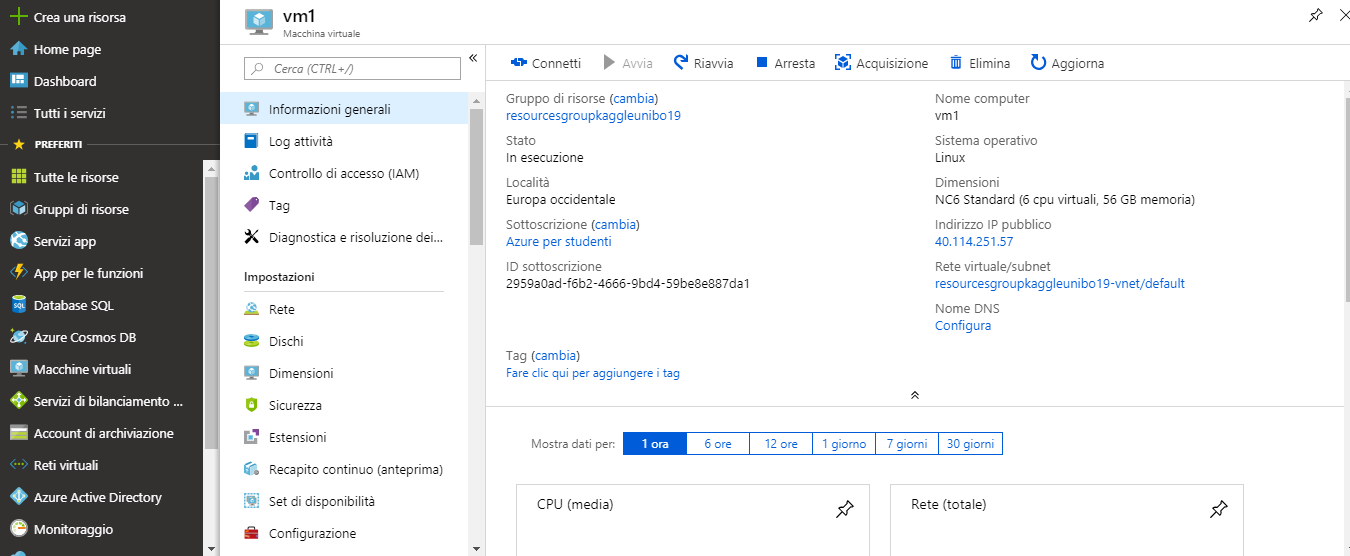
\includegraphics[width=0.9\linewidth]{pictures/azure.png}
	\caption{Azure Platform screenshot.}
	\label{fig:azure}
\end{figure}

According to the limitations given to student accounts, we instantiated the machine with the maximum of cores and GBs of RAM possible, which happened to be the NC6 Standard machine (with 6 virtual CPUs and 56 GBs RAM). Python was already installed on it, and we only had to install the other libraries (like \texttt{scikit-learn}) in order for our scripts to run. Access to the machine was made possible through SSH connection established through the \textit{PuTTY} client installed on our laptops \cite{putty}. Graphic visualization of the plots presented in the report were made available through \textit{Xming} \cite{xming}.

\begin{figure} [h]
	\centering
	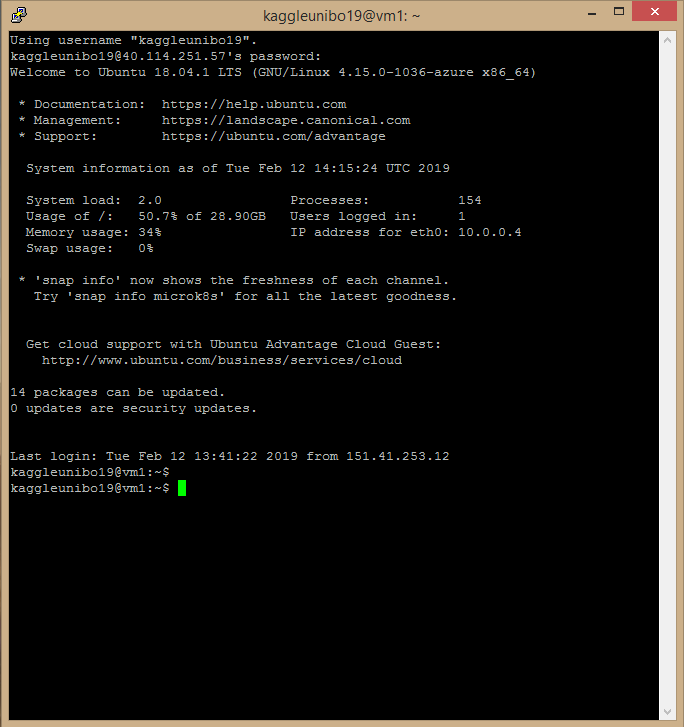
\includegraphics[width=0.7\linewidth]{pictures/cmd.png}
	\caption{Command line with SSH access to the VM.}
	\label{fig:cmd}
\end{figure}

The whole collection of \texttt{.py} scripts explored and the various results obtained have been saved and stored in a repository, available on GitHub \cite{github}.